\def\year{2021}\relax
\documentclass[letterpaper]{article}
\usepackage{adjustbox}
% DO NOT CHANGE THIS
\usepackage{aaai21}  % DO NOT CHANGE THIS
\usepackage{times}  % DO NOT CHANGE THIS
\usepackage{helvet} % DO NOT CHANGE THIS
\usepackage{courier}  % DO NOT CHANGE THIS
\usepackage[hyphens]{url}  % DO NOT CHANGE THIS
\usepackage{graphicx} % DO NOT CHANGE THIS
\urlstyle{rm} % DO NOT CHANGE THIS
\def\UrlFont{\rm}  % DO NOT CHANGE THIS
\usepackage{natbib}  % DO NOT CHANGE THIS AND DO NOT ADD ANY OPTIONS TO IT
\usepackage{caption} % DO NOT CHANGE THIS AND DO NOT ADD ANY OPTIONS TO IT
\frenchspacing  % DO NOT CHANGE THIS
\setlength{\pdfpagewidth}{8.5in}  % DO NOT CHANGE THIS
\setlength{\pdfpageheight}{11in}  % DO NOT CHANGE THIS


\setcounter{secnumdepth}{0} %May be changed to 1 or 2 if section numbers are desired.




\usepackage[utf8]{inputenc}
\usepackage[english]{babel}
\usepackage{amsthm}
\usepackage{amsmath}
\usepackage{amssymb}
\usepackage{graphicx}
\usepackage{xcolor}
\usepackage{bbm}
\usepackage{bm}
\usepackage{mathtools}
\usepackage{enumitem}
\usepackage{bbold}
\graphicspath{ {images/} }
\theoremstyle{definition}
\newtheorem{definition}{Definition}
\usepackage{caption}
\usepackage{subcaption}
\usepackage[rightcaption]{sidecap}
\usepackage[super]{nth}
\usepackage{wasysym}
\usepackage{multirow}
\usepackage{hhline}
\usepackage{algorithm}
\usepackage{algorithmic}
\usepackage{arydshln}
\newcommand{\argmax}[1]{\underset{#1}{\operatorname{arg}\,\operatorname{max}}\;}

\newcount\Comments  % 0 suppresses notes to selves in text
\Comments=0
\newcommand{\kibitz}[2]{\ifnum\Comments=1{\color{#1}{#2}}\fi}
\newcommand{\ym}[1]{\kibitz{blue}{[YM:#1]}}
\newcommand{\kg}[1]{\kibitz{red}{[KG:#1]}}
\newcommand{\li}[1]{\kibitz{brown}{[LL:#1]}}

\begin{document}

\title{Improving the Performance-Compatibility Tradeoff \\ with Personalized Objective Functions}

\author{
Jonathan Martinez,\textsuperscript{\rm 1}
Kobi Gal,\textsuperscript{\rm 1,2}
Ece Kamar,\textsuperscript{\rm 3}
Levi H. S. Lelis\textsuperscript{\rm 4,5}
\\
}
\affiliations{
\textsuperscript{\rm 1}Ben-Gurion University\\
\textsuperscript{\rm 2}University of Edinburgh\\
\textsuperscript{\rm 3}Microsoft Research\\
\textsuperscript{\rm 4}University of Alberta\\
\textsuperscript{\rm 5}Alberta Machine Intelligence Institute (Amii)\\
martijon@post.bgu.ac.il,
kobig@bgu.ac.il,
eckamar@microsoft.com,
levi.lelis@ualberta.ca
}

\maketitle
\bibliographystyle{aaai21}

\begin{abstract}
AI-systems that model and interact with their users can update their models over time to reflect new information and changes in the environment. Although these updates may improve the overall performance of the AI-system, they may actually hurt the performance with respect to individual users. Prior work has studied the tradeoff between improving the system's performance following an update and the compatibility of the updated system with prior user experience. The more the model is forced to be compatible with a prior version, the higher loss in performance it will incur. This paper  challenges this assumption by showing  that by
personalizing the loss function to specific users, it is possible to  increase the  prediction performance of the AI-system   while sacrificing  less   compatibility for these users.   Our approach updates the  sample weights  to reflect their contribution to the compatibility of the model  for a particular user following the update. We construct a portfolio of
different models that vary in how they personalize the loss function for a user. We select  the  best model
to use  for  a  target user based on a validation set.
We apply this approach to three supervised learning tasks commonly used in the human-computer decision-making literature. We show that using our approach leads to     significant improvements in the performance-compatibility tradeoff  over the  non-personalized approach of Bansal et al., achieving up to 300\% improvement    for certain users.  We present several use cases that illustrate the difference between the personalized and
non-personalized approach for two of our domains.
\end{abstract}
\section{Introduction}
\label{sec:intro}
Advancements in AI and ML have led to advice provisioning systems that derive insights and make predictions from large amounts of data. For example, expert diagnostic systems in healthcare predict patients' health condition by analyzing lifestyle, physical health records and social activities, and make suggestions to doctors about possible treatments~\cite{sahoo2019deepreco}.
As the user interacts with the system, two processes occur. First, the user develops a mental model of the system's capabilities based on the quality of the recommendations. Second, the system collects more data and is able to update its prediction models. While updating the system's model can improve its performance, it can also change the way the system makes predictions in a way that does not agree with the user's expectations, based on past interactions with the system. Thus while the update improves the overall system performance, it may exhibit a poor compatibility with the user's expectations~\cite{bansal2019updates}, possibly causing the user to lose trust in the system and ignore its recommendations. Or worse still, to follow wrong recommendations that the model prior to the update used to get right.

As an example, imagine a doctor that is being assisted by an AI-system that predicts whether skin moles are cancerous or not. Suppose that the system's average accuracy is currently 70\% overall, and that the doctor's specialty is face skin moles.
Next, the system  receives an update which increases its average accuracy to 90\% overall but decreases it to 60\% for face skin moles. As a consequence of this poorly compatible update, the doctor may notice the drop in accuracy regarding this specific region of data and start mistrusting the predictions of the system, therefore missing out on the benefits of being assisted by the AI-system.
Or worse still, the doctor may not notice this drop and therefore continue trusting the system's predictions that happen to be less accurate in this section of the data after the update.

Another example is an Intelligent Tutoring System that is sequencing math problems to students. The system predicts the student's performance on math problems with high accuracy. After an incompatible update, the system accuracy may increase overall but decrease when predicting student performance on Geometry questions, and as a result the system may ask the student redundant Geometry questions.

\citet{bansal2019updates} suggested a method for adjusting the compatibility of the model following an update to an AI-system  where the loss function is modified to incur an additional penalty for \textit{newly introduced mistakes}, i.e., mistakes that the system's updated version makes that the pre-update version didn't make. They show that a tradeoff exists between the compatibility and the performance of the updated model: The more it is forced to be compatible, the less accurate it will be.

A limitation in this approach is that all instances in the dataset are given the same importance regardless of their relevance to a particular user that interacts with the system.
In this paper we show that significant improvements in the performance-compatibility tradeoff can be achieved by \emph{personalizing} the objective function for   target users that interact with an AI-system. Our approach
weighs  each training sample with respect to its effect on the compatibility of the AI-system  following the update.
We  train different models that vary in the extent to which they personalize the  objective  function for
target users, including an extreme approach to personalization where the model relies exclusively on the personal history of the target user.

We apply this methodology towards computing the performance-compatibility tradeoff in  three domains from the human-computer decision making literature.
In each domain, we measure  the performance  of different personalization  models for  solving a classification  task according to  the area under the  performance-compatibility tradeoff curves ($AUTC$) that they produce.
Our  approach significantly outperformed the baseline approach \cite{bansal2019updates} in all domains in  terms of the $AUTC$ metric, achieving results that are as much as 90\% better on average and up to 300\% for certain users.
We  present several use cases that illustrate the difference between the personalized and non-personalized approach for two  of our domains.

These results carry important insights  for the designers of  AI-systems that interact with users over time. They  show that  by utilizing personalized objective functions to update the system, it is possible to improve the system's performance while minimizing the degradation of its compatibility with the model prior to the update.

\section{Preliminaries}
\label{sec:adjusting_comp}

Let $h_1$ be the model prior to the update and $h_2$ the model following the update, such that $h_1$ is trained on a small subset of the data used for training $h_2$. A newly introduced error is an error that $h_2$ makes that $h_1$ doesn't make.
The compatibility of an update to a classifier measures the amount of new errors that are introduced by the updated model  $h_2$.
\citet{bansal2019updates} propose the following definition for the compatibility score of an update:
\begin{definition}{The \textit{compatibility score} of a model $h_2$ relative to a pre-updated  model $h_1$ on some dataset $D$:}
\begin{equation}
\label{eq:compatibility}
C(h_1,h_2,D)=\frac{\sum_{i=1}^{|D|}\mathbb{1}[h_1(x_i)=h_2(x_i)=y_i]}{\sum_{i=1}^{|D|}\mathbb{1}[h_1(x_i)=y_i]}
\end{equation}
\end{definition}
\noindent Where $\mathbb{1}$ is the indicator function. The compatibility score is the ratio of samples in $D$ that $h_2$ predicts correctly among all the samples that $h_1$ predicts correctly. As the number of  newly introduced errors decreases the compatibility score approaches 1 and as this number increases it approaches 0.

\citet{bansal2019updates} propose a way of modifying a loss function $L$ (e.g., Cross-Entropy Loss) such that the amount of penalty given for the predicted label of an instance depends on whether it corresponds to a newly introduced error:
\begin{equation}
\label{eqn:non-personalized_loss}
L_c(x)=(1 - \lambda) \cdot
L(x)+\lambda\cdot
L(x)\cdot\mathbb{1}[h_1(x)=y]
\end{equation}
Where $L(x)$ is the penalty (loss) given to an updated model for the label it predicts for an instance $x$ and $\lambda\in [0,1]$ is the importance given to compatibility. We added the $(1-\lambda)$ term so that the whole spectrum of loss functions $L_c$ could be achieved by values of $\lambda$ that are between 0 and 1. We assume that the performance of  model $h_2$  on a held out test-set is at least as good as the performance of model $h_1$, which is a reasonable assumption since $h_2$ is trained on a superset of the data used to train $h_1$.

As the value of the parameter $\lambda$ increases, so does the  penalty for newly introduced errors. This simultaneously increases the compatibility score of the updated model and tends to decrease its performance as the updated model $h_2$ is forced to make predictions similar to those made by the pre-update model $h_1$. Varying the value of $\lambda$ generates a \emph{performance-compatibility tradeoff curve}, as depicted by the synthetic example shown in Figure~\ref{fig:example_tradeoff}.  The goal of the personalization approach we propose is to maximize the area under this curve, which is proportional to the quality of the tradeoff described by the curve.

\begin{figure}[t]
\centering
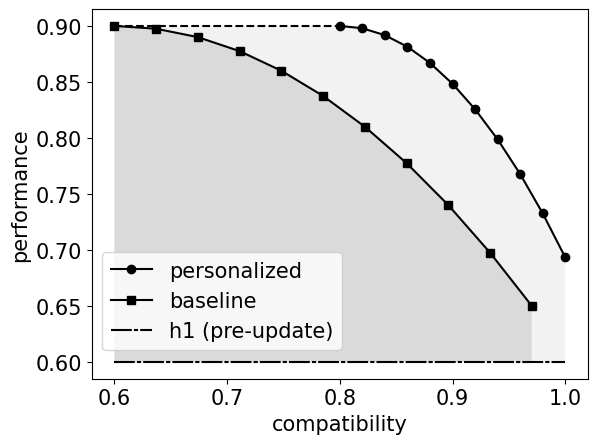
\includegraphics[width=0.45\textwidth]{example_tradeoff}
\caption{A synthetic example of performance-compatibility tradeoff curves. The x-axis represents the model's compatibility score (Equation~\ref{eq:compatibility}) and the y-axis its performance (e.g., accuracy). The dashed horizontal line corresponds to the performance of the pre-updated model $h_1$ while the curves correspond to two updated models fitted using Equation~\ref{eqn:sample_weights} with different vectors $W$. Each point corresponds to a particular value of $\lambda$ (the compatibility importance parameter).
}
\label{fig:example_tradeoff}
\end{figure}
In our medical example, once the modified loss function $L_c$ from Equation~\ref{eqn:non-personalized_loss} is used instead of the regular loss $L$ to update the system, there will be fewer newly introduced mistakes. This will improve the compatibility of the update at a certain expense of the system's overall accuracy, increasing the likelihood that the doctor will continue trusting the system's predictions.
\section{Personalizing Objective Functions}
\label{sec:personalization}

Our hypothesis is that personalizing the objective function for a particular user is likely to improve the performance-compatibility tradeoff provided to that user following the update to the system.

\begin{definition}
Hypothesis  $h$  is correct for  dataset $D$ if
$\forall x_i \in D$ we have that $h(x_i)=y_i$
\label{def:hypCorrect}
\end{definition}
Let $D$ be a dataset and $D^c\subseteq D$ be the subset of samples for which $h_1$ is correct. Errors that $h_2$ makes on samples in $D^c$ decrease its compatibility score, hence the superscript $c$ that stands for ``compatibility". Given a dataset $D$ and a pre-update model $h_1$ used to determine $D^c$, the weight of each sample $x\in D$ can be assigned by the following function:
\begin{align}
\label{eqn:non-personalized_sample_weights}
w_c(x,D,\lambda)&=(1-\lambda)\cdot\mathbb{1}[x\in D]+\lambda\cdot\mathbb{1}[x\in D^c] \\  \nonumber
&=(1-\lambda) + \lambda\cdot\mathbb{1}[x\in D^c]
\end{align}
Note that $\mathbb{1}[x\in D]$ is always equal to $1$, therefore we can simplify Equation~\ref{eqn:non-personalized_sample_weights} like shown above. Let $L_s$ be the summation of the penalties given by a loss function $L$ to the samples $x\in D$ weighted by some arbitrary weighting function $w$:
\begin{equation}
\label{eqn:loss_summation}
L_s(D,w) = \sum_{x \in D} w \cdot L(x)
\end{equation}
The objective function that results from summing the penalties given by $L_c$ (Equation~\ref{eqn:non-personalized_loss}) is equivalent to the one that results from using $w_c$ (Equation~\ref{eqn:non-personalized_sample_weights}) on $L_s$:
\begin{equation}
\label{eqn:Ls_equals_Lc}
L_s(D,w_c) = \sum_{x \in D}L_c(x)
\end{equation}
This means that utilizing $L_c$ is equivalent to assigning sample weights according to $w_c$ and utilizing the regular loss function $L$. Next, we extend Equation~\ref{eqn:non-personalized_sample_weights} to  \textit{personalize} the objective function for  particular users.
Let $D_i\subseteq D$ be the set of samples corresponding to the  history of interaction between user $i$ and the AI-system, and $D_i^c \subseteq D_i$ be the subset of those samples such that
the pre-update hypothesis $h_1$ is correct (Definition~\ref{def:hypCorrect}). As with $D^c$, errors that the updated model $h_2$ makes on $D_i^c$ are \textit{newly introduced errors} that reduce its compatibility score (Equation~\ref{eq:compatibility}).



\li{Assign a weight to each training instance? In which context? Perhaps we need to introduce an objective function so that this becomes easier to understand?}\ym{I changed the paragraph, maybe the issue is gone now}
We personalize the objective function to a target user  by assigning a weight to each sample in the dataset according to the following. Let $W=(w_0,w_1,w_2,w_3)$ be a set of four weights such that each weight captures the impact that each set of samples $D$, $D_i$, $D^c$ and $D_i^c$ (respectively) will have on the updated model's compatibility in respect to a target user $i$. \li{How about we write mnemonic subscripts to the weights? $w, w_i, w_c, w_{i,c}$?} \ym{nice idea! but maybe the $i$ in the subscript will be confusing? since it's not actually related to user $i$} Each combination of weights $W$ represents a different approach or degree of personalization. Given a dataset $D$, a target user $i$, a vector $W$ and a pre-update model $h_1$ used to determine both $D^c$ and $D_i^c$, we assign the weight to each sample $x\in D$ by the following function:
\begin{equation}
\label{eqn:sample_weights}
\begin{aligned}
&w(x,i,D,W,\lambda)=\\&(1-\lambda)\cdot (w_0\cdot \mathbb{1}[x\in D]+w_1\cdot \mathbb{1}[x\in D_i])\\&+\lambda\cdot (w_2\cdot \mathbb{1}[x\in D^c]+w_3\cdot \mathbb{1}[x\in D_i^c])
\end{aligned}
\end{equation}
\li{The $(1 - \lambda)$ is the performance term of the function; the $\lambda$ is the compatibility term of the function.}\ym{this distinction should first come when talking about Equation~\ref{eqn:non-personalized_loss}, so as I'm not sure how much has to be changed to accomodate this and this distinction is onlt really needed to explain why some values of $W$ fail at producing a tradeoff, I will simply make that explanation clearer for now}
By assigning the sample weights in this manner, we \emph{personalize} the objective function with respect to the target user $i$ according to the personalization approach indicated by $W$.
As in Equation~\ref{eqn:non-personalized_sample_weights}, the parameter $\lambda$ determines the importance the model gives to achieving a good compatibility score, therefore influencing the tradeoff between compatibility and performance.

Importantly, the personalized approach learns from the entire data set. But in contrast to the baseline approach, it distinguishes between the samples that belong to the target user's history and the ones that don't.
For instance, if a sample $x$ belongs to the target user $i$, then  $x\in D$ and $x\in D_i$, but $x \in D^c$ and $x\in D^c_i$ only if the pre-update model $h_1$ predicts the correct label for $x$.

As previously mentioned, by varying the weight parameters in $W$ we can generate models that differ in the extent to which the objective function is personalized to a target user. Let a model $m_k$ be a model fitted using the objective function that results from a given set of weights $W_k$. In this work we consider only binary weights (0 or 1), resulting in the family of models shown in Table~\ref{tab:models}.

\li{I don't understand what comes next. Once we polish this explanation we should probably move it to the end of the previous paragraph. The reader will be asking the question of where are the other models in the table 1 as soon as we mention it.}\ym{moved it, but I'm not sure how to improve it} Note that for some combinations of $W$ varying the value of  $\lambda$ will not change the weights of the samples relative to one another. Such models cannot generate a performance-compatibility tradeoff curve by varying the parameter $\lambda$ since varying it won't change their predictions in any way. Therefore, they are not included in the set of models $M$ we tested throughout the experiments. For example, $W=(1,1,0,0)$ collapses the weight function from Equation~\ref{eqn:sample_weights} into $(1-\lambda)\cdot (w_0\cdot \mathbb{1}[x\in D]+w_1\cdot \mathbb{1}[x\in D_i])$ that completely disregards compatibility as it ignores whether the pre-update model $h_1$ predicts the correct label.

\begin{table}
\begin{center}
{
\setlength{\tabcolsep}{4pt}
\begin{tabular}{c|cccc}
\hline
\rule{0pt}{6pt}
\multirow{2}{*}{model}&\multicolumn{4}{c}{$W_k$}\\
&$w_0$&$w_1$&$w_2$&$w_3$
\rule{0pt}{6pt}
\\\hline
$m_0$&1&0&1&0\\
$m_1$&0&1&0&1\\
$m_2$&0&1&1&0\\
$m_3$&0&1&1&1\\
$m_4$&1&0&0&1\\
$m_5$&1&1&0&1\\
$m_6$&1&0&1&1\\
$m_7$&1&1&1&0\\
$m_8$&1&1&1&1
\\\hline
\end{tabular}
\caption{The portfolio of models $M$.}
\label{tab:models}}
\end{center}
\end{table}

Each model represents a different approach to personalization. In particular, the model $m_0$ does not differentiate between users since its weight function is equivalent to Equation~\ref{eqn:non-personalized_sample_weights}.
This is the model of \citet{bansal2019beyond}, that we consider as our baseline.
In contrast, the objective function of $m_1$ represents an extreme approach to personalization where only the samples that belong to the user's history ($x\in D_i$) are considered.





















\section{Methodology}
\label{sec:methodology}
In this  section we present  our  methodology for selecting a personalized model for a target user and for measuring the quality of a performance-compatibility tradeoff.\footnote{Code and data  is publicly available  at~\url{https://github.com/jonmartz/CompatibilityPersonalization}}
To this end we interleave training the models $M$ for a given domain using a general purpose machine learning algorithm and  choosing the  best model for each user through a nested  cross-validation process~\cite{tashman2000out}.
This cross-validation process, described in Figure~\ref{fig:cross_validation}, preserves the temporal consistency of the user's interactions with the system and consists of two levels: An outer cross-validation loop for improving the statistical significance of the results and an inner cross-validation loop for selecting the best model for each user.

Let $D_i$ be the time-series data available for user $i$ in dataset $D$. In each outer-fold$_p$ a time-contiguous test set $Y_i^p\in D_i$ (10\% in our experiments) is chosen for each user $i$.
Let $D_i^p$ be the set of data points representing user $i$'s interactions that happened before all interactions in $Y_i^p$. We use $D_i^p$ for the inner cross-validation loop.
In each inner-fold$_{p,q}$ a timestamp is randomly selected for every user $i$ and used to split $D_i^p$ into disjoint and time-contiguous training set $T_i^{p,q}$ and validation set $V_i^{p,q}$.
We choose the timestamp defining the split randomly to vary the amount of training data for each user.
Every model $m_k\in M$ is trained on $T^{p,q}=\bigcup_j T_j^{p,q}$  and validated on $V_i^{p,q}$.
Each sample $x\in T^{p,q}$ is assigned the weight $w(x,i,T^{p,q},W_k,\lambda)$ (Equation~\ref{eqn:sample_weights} with the respective weight vector $W_k$ from Table~\ref{tab:models}).

The model with the best average performance on the sets $V_i^{p,q}$, where we vary $q$ and fix both $i$ and $p$, is chosen for the target user $i$.
Finally, we fit the chosen model on $D_i^p$, for maximizing the amount of training data, and evaluate it on the test set $Y_i^p$.
Each iteration of the outer loop provides a prediction and thus a quality metric of our system for user $i$.
We report the average results produced by the outer iterations of our cross-validation scheme.





\begin{figure}[t]
\centering
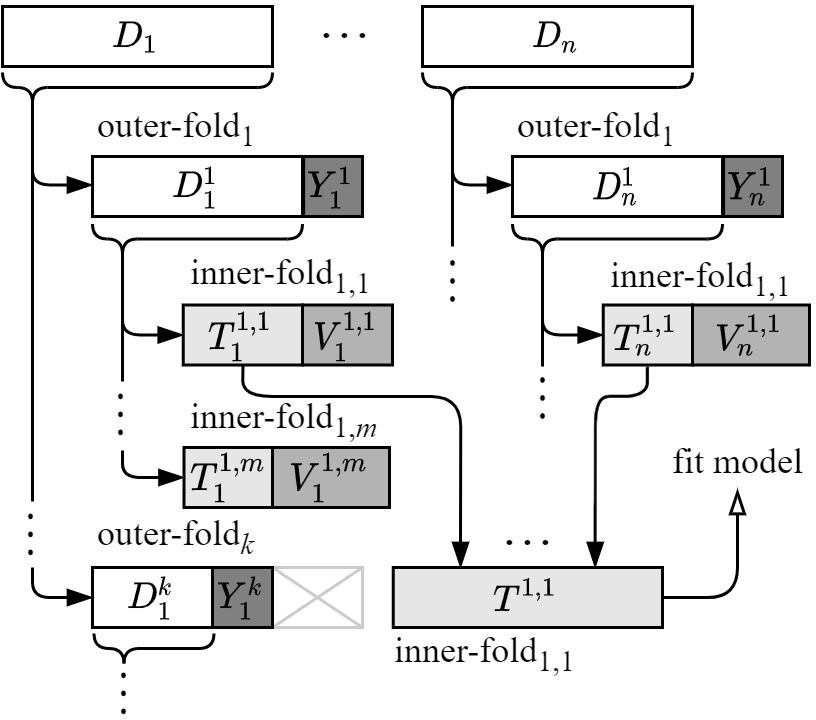
\includegraphics[width=0.45\textwidth]{cross_validation}
\caption{Visualization of the nested cross-validation employed in the experiments, with $k$ outer-folds, $m$ inner-folds and $n$ users. $D_i$ is the data of user $i$. In each outer-fold$_p$ a test set $Y_i^p$ is selected, while in each inner-fold$_{p,q}$ the remaining data $D_i^p$ is split into a train set $T_i^{p,q}$ and a validation set $V_i^{p,q}$. The models are fitted on $T^{p,q}$ (the union of all the user train sets). The crossed boxes indicate the data dropped as part of the cross-validation process.}
\label{fig:cross_validation}
\end{figure}

To evaluate a model we need to measure the quality of the performance-compatibility tradeoff it provides.
The  ROC curve (receiver operating characteristic curve) is a graph that shows the tradeoff between true positive and false positive ratios of a classification model's predictions, and the area under this curve -- commonly referred to as AUC -- provides a measure of the model's performance.
Similarly, to measure the quality of a performance-compatibility tradeoff we compute the  area under its curve (Figure~\ref{fig:example_tradeoff}), and call this metric AUTC (Area Under the Tradeoff Curve). The measure of model performance (y-axis in Figure~\ref{fig:example_tradeoff}) we report in our results is the aforementioned AUC.

An issue when comparing tradeoff curves by the AUTC metric is that one curve may start at a higher compatibility score than the other.
For example, in Figure~\ref{fig:example_tradeoff}, the starting points of the curves differ significantly in terms of compatibility, while the maximum compatibility scores they achieve are very similar.
This causes the area under the personalized model to be smaller than the area for the baseline, while clearly the tradeoff provided by the personalized model is better.
To correct this issue, we artificially extend the curves to the minimal compatibility score achieved by either one of the curves being compared.

For instance, in  Figure~\ref{fig:example_tradeoff} the personalized model provides a performance of 0.9 for its minimal compatibility score of 0.8, so we extend its curve with a straight line from compatibility score 0.8 to 0.6 in order to match the minimal compatibility score of the baseline (as indicated by the dashed line at the top of the plot). We report the area under the extended curve for the evaluated models, after removing the area below the line that corresponds to the performance of $h_1$ (the dashed line at the bottom of Figure~\ref{fig:example_tradeoff}) as we are interested only in improvements relative to the pre-update model's performance.












\section{Empirical Results}
\label{sec:results}

We applied our approach to three domains  commonly  used  in
Human-Computer Decision Making. \li{Why capitalize Human-Computer Decision-Making?}

\begin{enumerate}
\item   ASSISTments (available from PSLC Datashop \url{https://pslcdatashop.web.cmu.edu/}). This domain
includes interactions of students  solving online math problems in classrooms. The classification task is to predict if a student will answer a question  correctly on the first attempt given the history of the student's interactions with the system~\cite{feng2006addressing}.
The experiment included $\sim$50,000 instances from 100 students with histories ranging from 50 to 1000 instances with a mean of 525.

\item   Galaxy Zoo  (GZ)    (available from \url{https://data.galaxyzoo.org/}). This domain includes interactions from a crowdsourced astronomy project which invites people to assist in the morphological classification of large numbers of galaxies from digital images.  The classification task is to predict if a user
will dropout from the GZ site within a designated time window. We included $\sim$50,000 instances from 100 students with histories ranging from 50 to 1000 instances with a mean of 525.


\item The Stanford MOOCPosts (MOOC) dataset (available from https://datastage.stanford.edu/StanfordMoocPosts/). This domain  includes instances of   online forum posts of students from eleven Stanford University   courses. The  classification task is to predict if a forum post by a student reflects a high level of confusion about course material. The experiment included $\sim$5000 instances from 100 students with histories ranging from 20 to 500 instances with a mean of 260 (the longest histories found).

\end{enumerate}
Our criteria for selecting domains was that they 1) include multiple interactions between users and systems (e.g., classifying galaxies); 2) require  the system to make decisions in real time (e.g., determine whether a post is expressing confusion); \li{In this example the system is making decisions in real time, not the user. Maybe you meant that the system has to make decisions in real time?} 3) AI-systems can be potentially used to support the decision making of users (e.g., generating feedback to students).
\begin{figure}[t]
\centering
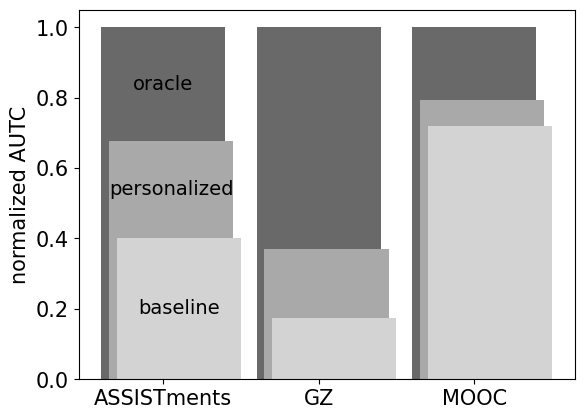
\includegraphics[width=8cm]{bar_graph}
\caption{Normalized AUTC measure for the baseline, personalized and oracle models on the different datasets. In all the paired t-tests between the personalized and baseline models the p-value was smaller than $0.05$.}
\label{fig:bar_graph}
\end{figure}
\begin{table}[t]
\begin{center}
{
\setlength{\tabcolsep}{4pt}
\begin{tabular}{c|cc}
\hline
\rule{0pt}{12pt}
\multirow{2}{*}{Dataset}&\multicolumn{2}{c}{\% times better than baseline}\\
\rule{0pt}{12pt}
& Personalized& Oracle
\\\hline
\rule{0pt}{12pt}ASSISTments&$26.4\%$&$62.8\%$\\
\rule{0pt}{12pt}GZ&$16.2\%$&$30.4\%$\\
\rule{0pt}{12pt}MOOC&$15.9\%$&$40.4\%$\\
\hline
\end{tabular}
\caption{Percentage of times that our approach and an Oracle with hindsight selected a model that performed better (not equal) than the baseline in a test set.}
\label{tab:agent_results}}
\end{center}
\end{table}

We trained the models in $M$ (Table~\ref{tab:models}) using the version of decision tree classifiers (CART) implemented in the scikit-learn Python package \cite{scikit-learn}. Each model is trained multiple times with various values of $\lambda$ to produce the tradeoff curves.
We  used the ``sample\_weights" parameter to personalize the sample weights  according to Equation~\ref{eqn:sample_weights}.\footnote{Neural Networks provided a better performance than the Decision Trees, but we decided to report results for the latter because it is more explainable to people.}

Figure~\ref{fig:bar_graph} shows results averaged over all the users and all the cross-validation folds in each dataset. The height of each bar indicates the model's AUTC divided by the AUTC of an Oracle model that has hindsight of which model is best for each user's set (has full information).
The difference between the personalized model and the baseline is statistically significant (obtained a p-value below $0.05$ on a paired t-test between the two models, on all three datasets).

Table~\ref{tab:agent_results} shows the percentage of times that the personalization approach and the Oracle outperformed the baseline. These results indicate that there's still room for improving the personalization approach and achieving a performance closer to that of the Oracle. For instance, in the ASSISTments dataset the personalized approach selected a model that is better than the baseline $26.4\%$ of the time while the Oracle did so $62.8\%$ of the time.

\begin{figure}
\centering
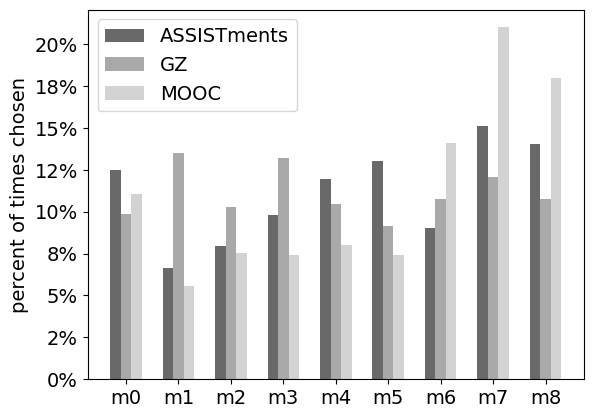
\includegraphics[width=0.47\textwidth]{model_counts}
\caption{Histogram of the amount of times each model $m\in M$ was the best performing one in a user's validation set.}
\label{fig:model_counts}
\end{figure}

\begin{figure*}[t]
\begin{subfigure}[b]{.4\textwidth}
\centering
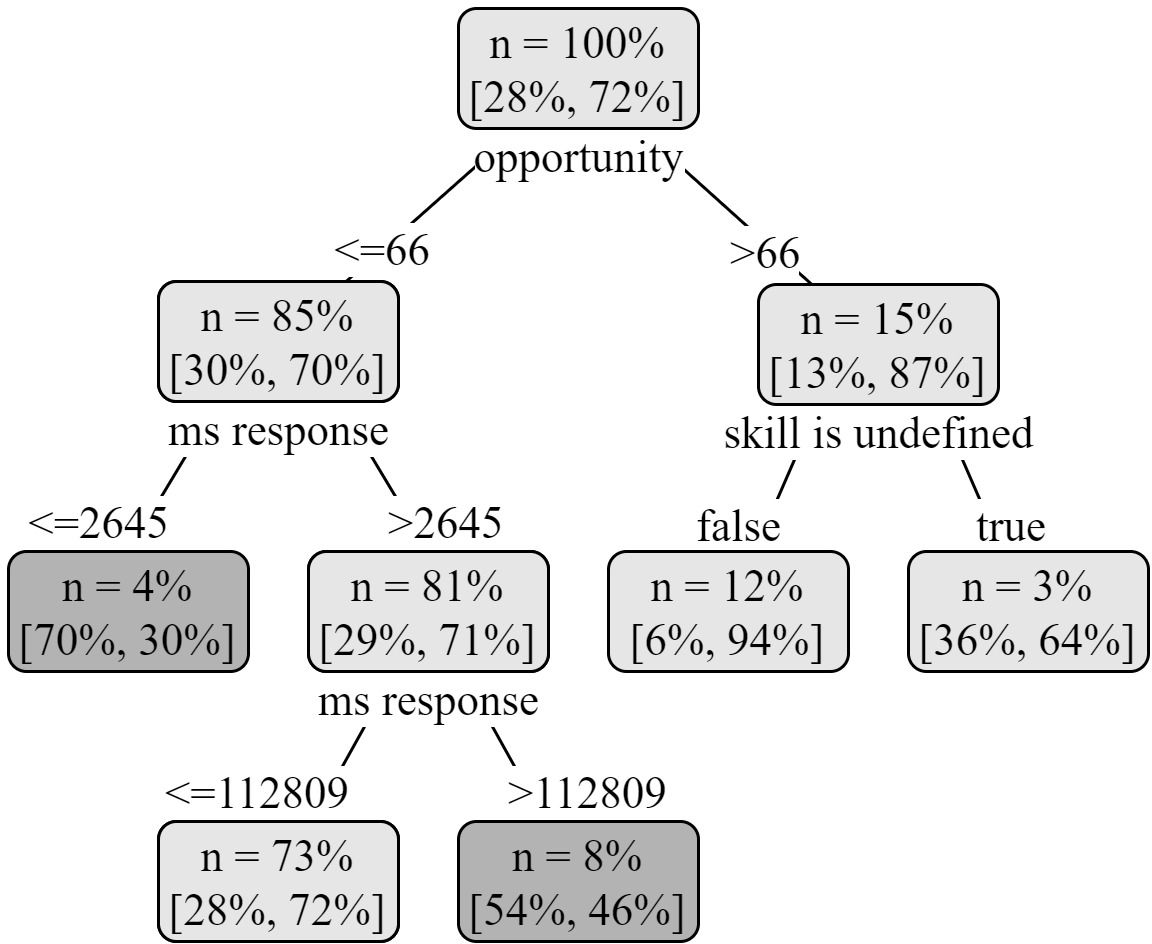
\includegraphics[width=0.95\linewidth]{assistments_baseline}
\caption{Baseline (compatibility $=88\%$, AUC $=54\%$)}
\label{fig:assistments_baseline}
\end{subfigure}
\begin{subfigure}[b]{.6\textwidth}
\centering
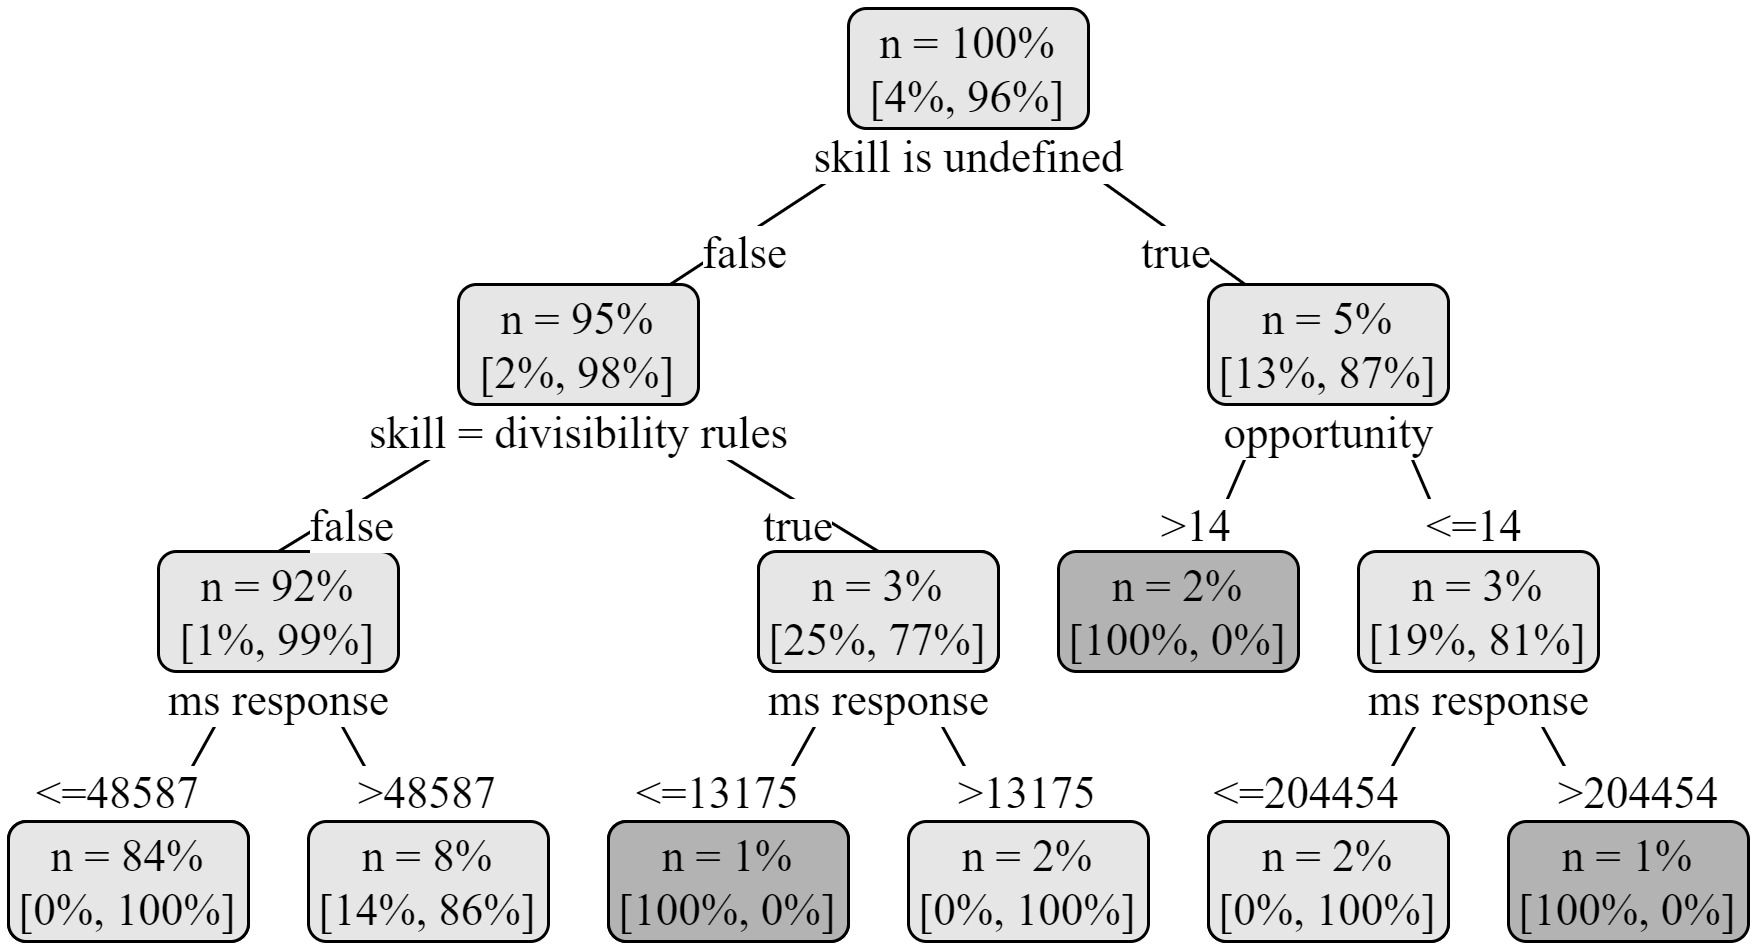
\includegraphics[width=0.95\linewidth]{assistments_personalized}
\caption{Personalized (compatibility $=94\%$, AUC $=62\%$)}
\label{fig:assistments_personalized}
\end{subfigure}
\caption{Baseline and personalized decision trees (up to a depth of 3) for a target user in the ASSISTments dataset,  produced by the CART algorithm.  Each node includes  the percentage of training samples at the respective node and the distribution over the target class weighted according to the sample weights (the shade indicates the majority class). The performance and compatibility measures in the user's test set are indicated.}
\label{fig:user_case_assistments}
\end{figure*}

Figure~\ref{fig:model_counts} shows the percentage of times each model from $M$ was the best model in a user's validation set. This distribution indicates that no model is always better than all the others, and that even the baseline ($m_0$) is sometimes the best model.
The model $m_7$ performed best most of the time in the ASSISTments and MOOC datasets, while the model $m_1$ did so in the GZ dataset. This indicates that in the two former datasets it was preferable to consider all the users (as $m_7$ assigns a non-zero weight to all the samples) while in the GZ dataset it was better to consider only the target user (as $m_1$ assigns zero weight to all the samples that come from non-target users).

Selecting the best model for each user using the inner cross-validation depicted in Figure~\ref{fig:cross_validation} proved to be a significantly better strategy than naively selecting one of the models in $M$ to be used uniformly on all the users in a dataset. Doing so without the cross-validation didn't yield statistically significant improvements relative to the baseline due to high variance in the results.

\subsection{Use Cases}
\label{sec:user_cases}
In this section we present two use cases in which the personalized model differed from the baseline model of Bansal et al.~\shortcite{bansal2019beyond} and provided a better performance-compatibility tradeoff.
In each case, we describe the difference between a decision tree produced by the baseline model ($m_0$) and one produced by the personalized model (selected using the user's validation sets) such that both its compatibility and performance are significantly better than the baseline model.
We focus on describing the differences between the models.

We begin with the ASSISTments dataset, where the classification task is to predict whether a student will solve a math problem correctly or not.  The baseline model and the personalized model for the target user are shown in Figure~\ref{fig:user_case_assistments}.
The model that provided the best tradeoffs in average on this user's validation sets was $m_5$, which also happened to achieve a significantly better performance-compatibility tradeoff than $m_0$ (the baseline model) on the user's test set.


A significant difference is that the personalized model uses the fact that the student lacks knowledge regarding some skills (``divisibility rules" and ``least common multiple") as the student tends to choose the wrong answer in questions involving these skills, while the baseline model does not consider any particular skill.

An important  trend that is  exhibited in  the dataset is that if a student's response time is less than $\sim$3000 milliseconds the answer is very likely to be incorrect.
According to an ASSISTments domain expert, a possible reason for this is that a short response time indicates that the student has guessed the answer.
The baseline model capitalizes on this trend, significantly basing its decisions on this threshold.
On the other hand, the personalized model did not split on this variable, possibly reflecting the fact that it's less common for the target user to guess an answer.

The ``opportunity" variable indicates how many questions involving the same skill the student has answered in the past.
According to domain experts, high opportunity values along with incorrect answers reflect students who are ``gaming'' the system and answering arbitrarily, since the number of opportunities stacks up with each answer given to questions involving the same skill regardless of its correctness.
The personalized model predicts the answer will be incorrect given an opportunity count greater than 14 on questions where the skill involved is not defined, hinting that this student may be a ``gamer" when it comes to this kind of questions. The baseline model does not check for this trend, possibly indicating that most students are not ``gamers".






Next we analyze a use case for the MOOC dataset, where the classification task is to predict whether a forum post by a student reflects a high level of confusion or not. Please refer to the supplementary material to see the corresponding decision trees. The personalized model significantly outperformed the baseline model in terms of AUC (97\% vs 68\%) when being 100\% compatible with the pre-update model. In this case the best performing model in the user's validation sets was $m_3$, a model that gives a relatively low importance to non-target users.

The most important difference between the baseline model and the personalized model is that the personalized model considers whether the forum post contains many words of the type ``insight" and ``cause", which are words like ``think", ``know" and ``because".
The fact that a post includes many of these words indicates that the student may be explaining something rather than posting a question that expresses confusion.
The personalized model benefited from making this distinction, which it found useful apparently because the target student commonly gives explanations to other students.

Another difference between the two models is that the  the personalized model's decision tree branches according to the amount of words in the category ``tentative", which includes words like ``maybe" and ``perhaps". In the cases where the student included many of these words, the forum post was likely to indicate confusion.
The baseline tree doesn't branch by this variable, possibly indicating that this student hypothesizes answers to his/her own questions more often than the average user.

Lastly, the personalized model's tree checks for whether the post includes many words from the ``friend" category, which are words like ``buddy" and ``neighbor". It found that the post is very likely not showing confusion if it contains many of these words, which may indicate that this student often engages in social conversations.
\section{Related Work}

This paper builds on the recent work of \citet{bansal2019updates} that introduces the idea of the compatibility score of an update (Equation~\ref{eq:compatibility}) and proposes a method for increasing this score by employing a customized loss function (Equation~\ref{eqn:non-personalized_loss}) where an additional weighted penalty is given for newly introduced errors (mistakes that the model prior to the update didn't make). They showed that forcing the update to be more compatible generally decreases its performance, i.e. a performance-compatibility tradeoff. We expand this method by adding the notion of personalization towards target users with the goal of improving the performance-compatibility tradeoff provided by the update. % (i.e., with a larger AUTC, see Definition~\ref{def:AUTC}).  The underlying idea behind the method proposed by \citet{bansal2019updates} (and therefore behind the method proposed here as well) is similar to several other works. One such example are Model Ensemble methods \cite{opitz1999popular}, in particular AdaBoost \cite{freund1996experiments}. In both methods, an additional penalty is given for different types of errors that depends on a previously trained model. In AdaBoost this additional penalty is given for mistakes that the previous model made and in the method of \citet{bansal2019updates} for mistakes the previous model didn't make.
It could be interesting to explore the theoretical similarities between these two methods, since model ensemble enjoys a vast theoretical framework \cite{freund1996experiments}.

Choosing the best model for each user is related to research on methods for choosing the best expert \cite{herbster1998tracking}, but in our work we simply consider the quality of the performance-compatibility tradeoffs (in terms of AUTC) provided by the various models on a validation set to determine this.
Further implementation of the ideas proposed in that research may improve the reliability of this selection.

Several other works relate to the personalization of AI-models to users but do not address the personalization of updates to these systems, let alone the notion of an update's compatibility with the prior model. For instance, for the ASSISTment dataset mentioned in previous sections, work was performed on individualizing student models  \cite{wang2012student,pardos2010modeling} and on clustering the students \cite{trivedi2011clustering,trivedi2010spectral} with the goal of improving the accuracy of the predictions.

Much work has been done in the field of human-AI interactions. The compatibility of an update to an AI-system is closely related to the \nth{14} Guideline for Human-AI Interactions from Amershi et al.'s work \cite{amershi2019guidelines} described as \emph{``Update and adapt cautiously: Limit disruptive changes when updating and adapting the
AI-systems behaviors''}. In our case, this means making sure that the predictions made by the updated model conform to the user's expectations that developed prior to the update. It is related also to the \nth{5} step in an article from Google Design \cite{lovejoy2017} that states the importance of making sure that the AI-system and the user's model evolve in tandem. For more references to related work on human-AI interaction and the field of AI-advised human decision making refer to the related work section in the paper of \citet{bansal2019updates}.
\vspace{-0.92mm}
\section{Conclusion}
The compatibility of an update to an AI-system with the system prior to the update is important for the adequate functioning of human-AI teams \cite{bansal2019beyond, bansal2019updates}. Previous work addressed the problem of increasing compatibility by developing a loss function that delivers an additional penalty for newly introduced errors (mistakes that the model prior to the update didnt make), and showed that there's a tradeoff between the compatibility and performance of the updated model \cite{bansal2019updates}. We extended this approach by personalizing the model's objective function to target users with the goal of producing improving this tradeoff. We also proposed a framework for selecting the best way of performing this personalization.

The experimental results showed that our personalization approach can yield significantly better performance-compatibility tradeoffs than the baseline non-personalized model.
We then analyzed two use cases where the personalization exceptionally outperformed the baseline and showed that the personalized classifier model differed fundamentally from the baseline model.

Our approach is limited in the sense that it assumes that the user's future interactions with the system will resemble the ones observed so far.
In future work we will address this limitation, and explore ways of modifying the objective function beyond simply assigning weights to the dataset samples possibly by employing program synthesis or inverse reinforcement learning methods. We believe that informing users  about the   performance-compatibility tradeoff  of the models that are used to interact with them can  contribute on making AI-systems more transparent.



\vspace{-0.75mm}
\section{Acknowledgements}
Thanks very much to Avi Segal and Nicholas Hoernle for helpful comments. This research was partially supported by Israeli Science Foundation (ISF) Grant No. 773/16 and by Canada's CIFAR AI Chairs program.


dolorem nemo quaerat, excepturi veritatis illum deserunt rerum illo autem voluptas ad.Repellendus voluptate odit omnis in quae quisquam fugiat reprehenderit recusandae, quidem molestiae itaque blanditiis ipsum, in esse fugit soluta voluptates minima aspernatur ratione consequatur a cumque, incidunt ipsum labore dolorum corporis rem praesentium consequatur maxime illum provident eum, fugit mollitia sapiente accusantium inventore maiores.Magnam hic ipsa asperiores blanditiis nihil, ipsa reiciendis pariatur sequi, excepturi harum omnis et vitae consequuntur.Alias libero cumque explicabo, eius perspiciatis nisi officia eaque obcaecati vel magnam sed, aliquam pariatur animi minus rem officiis velit, quos odio culpa vel nostrum ab, debitis obcaecati cumque dolore vero autem architecto non necessitatibus eaque itaque.Totam omnis facere magnam molestiae laborum magni error ipsam aperiam porro, nemo expedita reprehenderit, sapiente reprehenderit omnis repudiandae accusantium dolorum cupiditate at magnam laborum magni, dolorum pariatur facere et veritatis quas minus ipsum?Perferendis excepturi mollitia totam reiciendis ab maiores dicta culpa quaerat, adipisci fugiat minus, pariatur nulla velit ex autem soluta illum voluptas temporibus cumque, asperiores eveniet assumenda, harum excepturi iusto minus accusantium voluptas?Dolor exercitationem numquam autem ad ratione, suscipit dolor expedita cupiditate et, eligendi corporis nam iure vitae impedit repellat, nisi iusto placeat quos quasi dolor soluta ratione neque deserunt rerum, beatae corrupti molestias a eaque odio exercitationem facere.\clearpage
\bibliography{ecai}
\end{document}


